\documentclass[UTF8,a4paper,zihao=5,fontset=fandol]{ctexart}
\usepackage[margin=2.3cm]{geometry} % 页边距
\usepackage{lmodern}               % 可缩放的西文与数学字体
\usepackage{amsmath}               % 数学公式
\usepackage{booktabs}              % 三线表
\usepackage{graphicx}              % 插入图片
\usepackage{float}                 % [H] 表示图表放在当前位置
\usepackage[hidelinks]{hyperref}   % 交叉引用
\usepackage{titling}              % 紧凑的标题布局
\usepackage{xcolor}
\setlength{\droptitle}{-1.5cm}
\postdate{\par\end{center}\vspace{-1.5em}}
\linespread{1.05}
\ctexset{section={format=\large\bfseries,beforeskip=1ex,afterskip=0.6ex}}
\setlength{\intextsep}{8pt}

\title{题目四：BinarySearch 平均运行时间实验}
\author{姓名：\quad 学号：}
\date{} % 如需日期，可改为 \date{\today}

\begin{document}
\maketitle

\section{实验计划}
取 $n=1,2,5,10,20,30,40,50,60,70,80,90,100$，每个规模测试
$R=1000$ 次。每次从 $0\sim314$ 中随机抽取 $n$ 个互异整数并排序，
再从同一范围随机选取目标值。用 \textbf{perf\_counter\_ns()}
计时，{\color{red}{仅测量 \texttt{BinarySearch} 调用}}，不计数组生成和排序。

\begin{equation}
  t(n)=\sum_{i=1}^{R}\Delta t_i,
  \qquad R=1000.
\end{equation}


\section{实验结果}
实验环境为 Windows 11、Python 3.14.6。
测得的平均运行时间见表~\ref{tab:time}，变化趋势见图~\ref{fig:time}。


\begin{table}[H]
  \centering
  \renewcommand{\arraystretch}{0.90} % 调整表格行距
  \caption{不同数组长度下的平均运行时间}
  \label{tab:time} % label 放在 caption 后面
  \begin{tabular}{rr} % 两列，均右对齐
    \toprule
    数组长度 $n$ & 平均时间（$\mu\mathrm{s}$） \\
    \midrule
    1   & 0.2515 \\
    2   & 0.3110 \\
    5   & 0.4080 \\
    10  & 0.5120 \\
    20  & 0.6302 \\
    30  & 0.6219 \\
    40  & 0.6571 \\
    50  & 0.7638 \\
    60  & 0.6985 \\
    70  & 0.7143 \\
    80  & 0.7723 \\
    90  & 0.7358 \\
    100 & 0.7684 \\
    \bottomrule
  \end{tabular}
\end{table}

\begin{figure}[H]
  \centering
  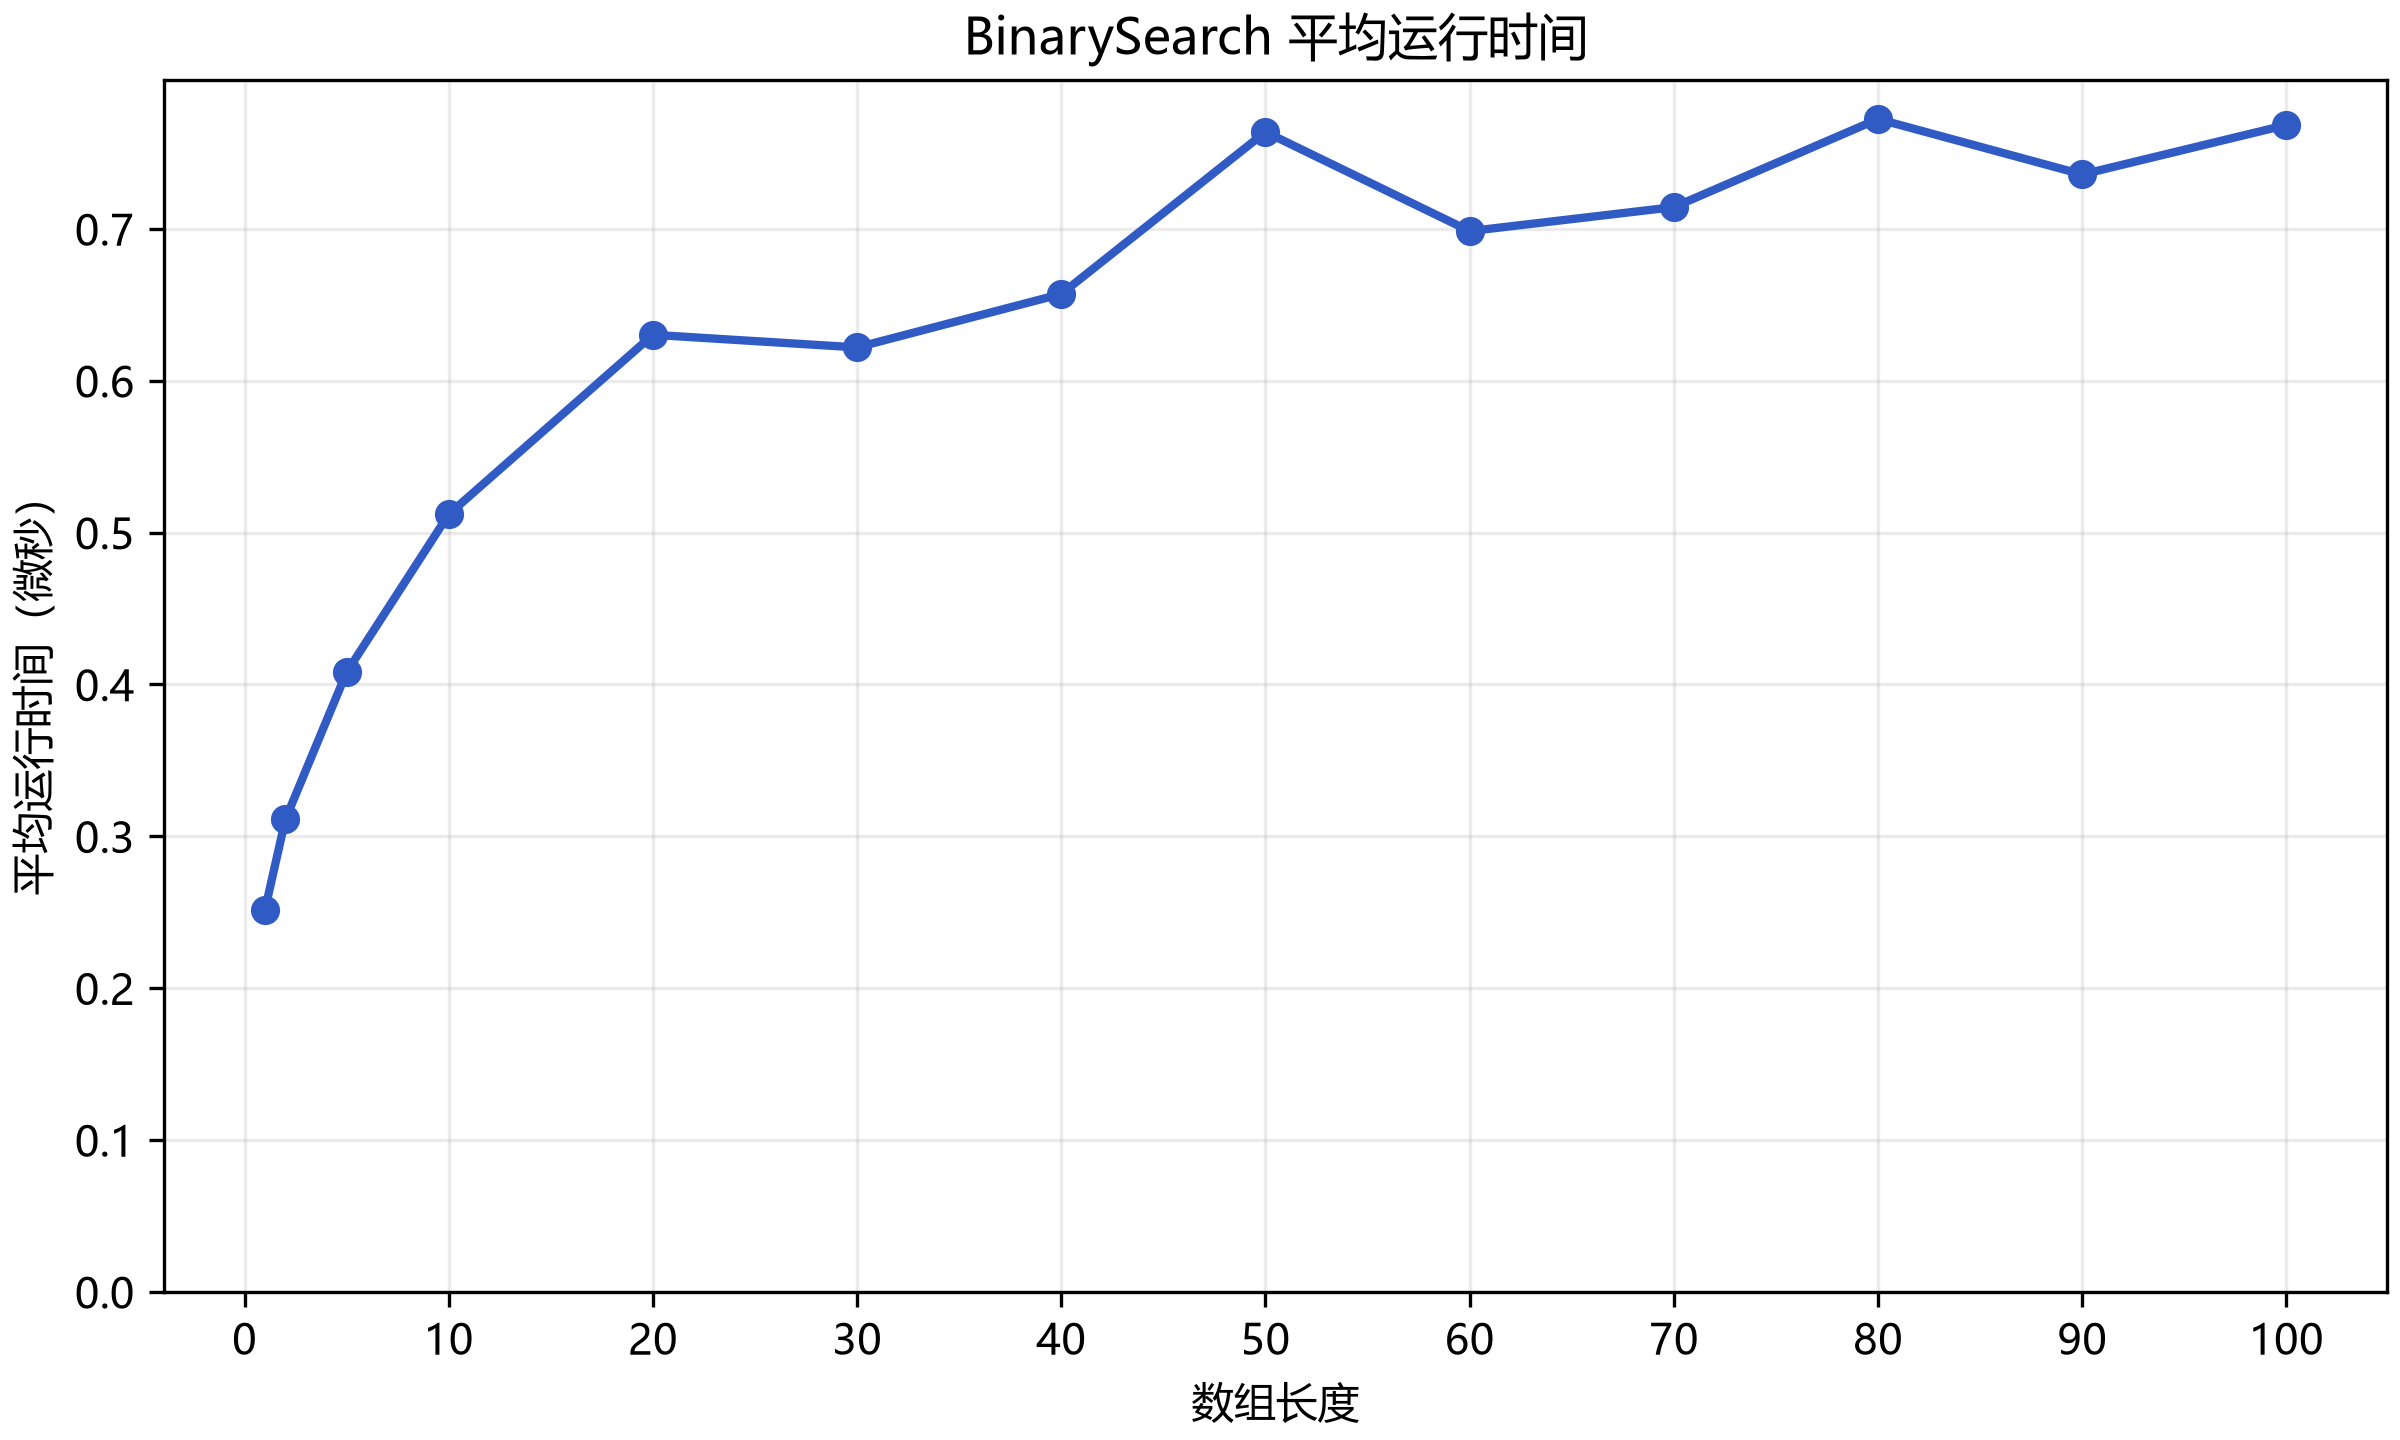
\includegraphics[width=0.62\linewidth]{Ex4_plot.png}
  \caption{BinarySearch 平均运行时间随数组长度的变化}
  \label{fig:time}
\end{figure}

\section{结果分析}
平均耗时总体随 $n$ 增大而上升，但存在局部波动。
二分查找每轮将搜索范围缩小约一半，理论时间复杂度为 $O(\log n)$。
实验包含成功与失败查找
值得指出的是，由于规模较小，计时开销和系统调度会影响结果，实测曲线不能单独证明复杂度。
\end{document}
